\documentclass[../report.tex]{subfiles}

\begin{document}

\begin{figure}
\centering
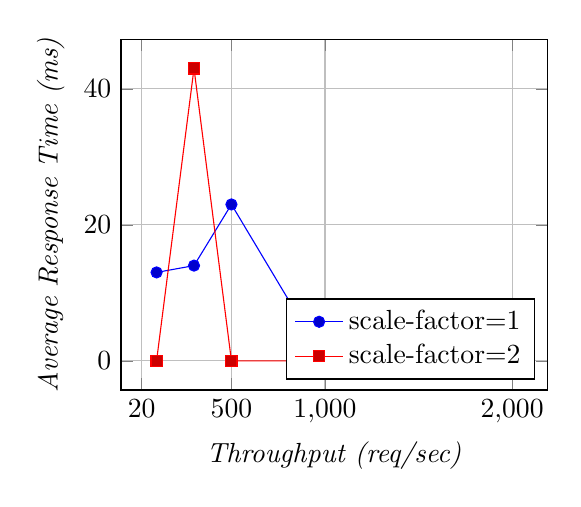
\begin{tikzpicture}[baseline]
    % \begin{axis}[width=7cm, xlabel=\emph{Throughput (req/sec)}, ylabel=\emph{System Load}, ylabel near ticks, grid=major, legend pos=south east, nodes near coords, every node near coord/.append style={font=\footnotesize}, every node near coord/.append style={yshift=-0.5cm}]
    \begin{axis}[width=7cm, xlabel=\emph{Throughput (req/sec)}, ylabel=\emph{Average Response Time (ms)}, ylabel near ticks, grid=major, legend pos=south east, xtick={20, 500, 1000, 2000}]
        \addplot coordinates {
            (2000,0) (1000,0) (500,23) (300,14) (100,13)
        };
        \addlegendentry{scale-factor=1}

        \addplot coordinates {
            (1000,0) (500,0) (300,43) (100,0)
        };
        \addlegendentry{scale-factor=2}
    \end{axis}
\end{tikzpicture}
\label{fig:pg_time}
\caption{Queries' runtime}
\end{figure}

\end{document}
